\documentclass[
	preprint,%twocolumn
	aps,
	prb,
	showpacs,	
	amsmath, amssymb]{revtex4-2}
%---packages----------------------------------------------------------
%\usepackage[top=1.25in, bottom=1.25in, left=1.25in, right=1.25in]{geometry}
\usepackage{bm}
\usepackage{graphicx}
\usepackage{hyperref}% add hypertext capabilities
\hypersetup{colorlinks=true, 
			citecolor=blue, 
			urlcolor=blue, 
			linkcolor=blue}
\pdfstringdefDisableCommands{\let\bm=\relax}
\usepackage{scalerel}
\usepackage{cleveref}
\usepackage{tikz} % flow chart
\usetikzlibrary{positioning, shapes.geometric}


%--setups--------------------------------------------------------------
\DeclareRobustCommand{\xjoinrel}{\mathrel{\mkern-4mu}}
\DeclareRobustCommand{\gong}{\hstretch{1.25} {\boldsymbol{\mathrel{|} \xjoinrel\mathrel{-} \xjoinrel\mathrel{|}}}}
%\DeclareRobustCommand{\gong}{\hstretch{1.25} {\boldsymbol{\vdash \xjoinrel\dashv }}}
%\DeclareRobustCommand{\wang}{\hstretch{1.25} {\boldsymbol{\vdash \xjoinrel \mathrel{+} \xjoinrel\dashv }}}
\DeclareRobustCommand{\wang}{\hstretch{1.25} {\boldsymbol{\mathrel{|}  \xjoinrel\mathrel{-} \xjoinrel\mathrel{|} \xjoinrel\mathrel{-} \xjoinrel\mathrel{|}}}}
\DeclareRobustCommand{\+}{\hstretch{1.25} {\boldsymbol {\mathrel{+}}}}
\DeclareRobustCommand{\manyplus}{\hstretch{1.25} {\boldsymbol{ \mathrel{+}\xjoinrel \mathrel{+}\xjoinrel\mathrel{+} \xjoinrel\mathrel{+}}  }}
\DeclareRobustCommand{\l}{\hstretch{1.25} {\boldsymbol {\vdash }}}
\DeclareRobustCommand{\r}{\hstretch{1.25} {\boldsymbol {\dashv }}}
%\DeclareRobustCommand{\tu}{\hstretch{1.25} {\boldsymbol {\mathrel{+} \xjoinrel\dashv }}}
\DeclareRobustCommand{\tu}{\hstretch{1.25} {\boldsymbol{\mathrel{-} \xjoinrel\mathrel{|} \xjoinrel\mathrel{-} \xjoinrel\mathrel{|}}}}
%\DeclareRobustCommand{\tl}{\hstretch{1.25} {\boldsymbol {\xjoinrel\dashv \mathrel{+}}}}
\DeclareRobustCommand{\tl}{\hstretch{1.25} {\boldsymbol{\mathrel{|}  \xjoinrel\mathrel{-} \xjoinrel\mathrel{|} \xjoinrel\mathrel{-} }}}

\newcommand{\tr}{ {\rm Tr} }
\newcommand{\I}{ {\mathbb I} }
\newcommand{\im}{ {\mathrm{Im}} }
\newcommand{\re}{ {\mathrm{Re}} }
\newcommand{\sgn}{ {\mathrm{Sgn}} }
\newcommand{\Y}{ {\mathcal{Y}} }
\newcommand{\C}{ {\mathcal{C}} }
\newcommand{\Cbar}{ {\bar{\mathcal{C}}} }
\newcommand{\D}{ {\mathcal{D}} }
\newcommand{\Dbar}{ {\bar{\mathcal{D}}} }
\newcommand{\B}{ {\mathcal{B}} }
\newcommand{\N}{ {\mathcal{N}} }

%=======================================================================
%=======================================================================
\begin{document}
\title{Notes: Nevanlinna analytical Continuation Method}
\author{Shuang Liang}
\email{sliang@iphy.ac.cn}
\affiliation{Institute of Physics, Chinese Academy of Sciences}


%\author{Shuang Liang}
%\affiliation{Institute of Physics, Chinese Academy of Sciences}
%\email{sliang@iphy.ac.cn}

\date{\today}
\begin{abstract}
	This is the abstract.
\end{abstract}


\maketitle
\tableofcontents

\newpage
%=====================================================================
%=====================================================================
\section{The analytic continuation problem}
\label{sec:the-analytic-continuation-problem}

The analytic continuation problem seeks   
to extract real frequency dynamical information from
imaginary-time correlation functions $G(\tau)$ data.
Technically, this is a highly nontirvial task\cite{jarrell1996bayesian}. To 
see this, we use the relation between $G(\tau)$ and $A(\omega)$
\cite{jarrell1996bayesian,XiaoLRT}:
\begin{equation}\label{eq:gt-Aw}
	G(\tau) = \int_{-\infty}^{\infty} d\omega
		\frac{e^{-\tau \omega }}{1 - \lambda e^{-\beta \omega}}
		A(\omega)
		= \int_{-\infty}^{\infty} d\omega
		K(\tau, \omega) A(\omega)
\end{equation}
where $K(\tau, \omega) = \frac{e^{-\tau \omega }}{1 - \lambda e^{-\beta \omega}}$
is the kernel, $\lambda =\pm 1$ for bosons/fermions respectively. One may consider to solve the problem by firstly 
discretize $\tau$ and $\omega$ and get:
\begin{equation}
	G(\tau_i) = \sum_{j=1}^{N_\omega} K_{ij} A(\omega_j)
\end{equation}
Then do SVD decomposition of rectangular matrix $K$, write
$K_ij = U_{il} \lambda_l V_{lj}$. Finally the spectral function 
reads
\begin{equation}
	A(\omega_j) = \sum_{l=1}^{N_\tau} \frac{1}{\lambda_l} V_{ij}
		\sum_{i=1}^{N_\omega} G(\tau_i) U_{il}
\end{equation}
It seems fine at the first glanse. However, if we consider 
the properties of $K(\tau, \omega)$, we would notice that it 
is highly sigular since it is exponentially small for large 
$|\omega|$, so small errors $G(\tau)$ would be amplified by
exponentially small $\lambda_l$. This problem is well-known
ill-posed\cite{acton1997numerical, peschel1999density} and 
enormous efforts have been made\cite{}.


%=====================================================================
%=====================================================================
\section{How to solve?}
\label{sec:how-to-solve}

$\cdots$

Here we introduce the recently developed Nevanlinna 
analytic continuation method\cite{fei2021nevanlinna}.      
%=====================================================================
%=====================================================================
\section{Nevanlinna analytic continuation method}
\label{sec:nevanlinna-analytical-continuation-method}

The Nevanlinna analytic continuation method\cite{fei2021nevanlinna} 
is an interpolation method. The key step is to build the conformal mappings 
from the open upper half of the complex plane $\C^+$ 
to a closed unit disk $\Dbar$ in the complex plane and 
make use of the Schur algorithm
\cite{schur1917potenzreihen,schur1918potenzreihen,dym2003contributions} 
to do the interpolate.

%=====================================================================
\subsection{Schur Algorithm}
\label{subsec:schur-algorithm}

Schur Algorithm was introduced by I. Schur\footnote{Schur 
	published under the name of both I. Schur, 
	and J. Schur, the latter especially in  
	\textit{Journal für die reine 
	und angewandte Mathematik}. This has led to some confusion.
	See:\href{https://en.wikipedia.org/wiki/Issai_Schur#cite_note-2}{Issai Schur}} 
in Section 1 of Ref.\cite{schur1917potenzreihen}.
Here we list the main results we need while
for a detailed introduction, see Ref.\cite{dym2003contributions}. 

A Schur class($\mathcal{S}$) consists of the Schur functions, which are the 
\href{https://en.wikipedia.org/wiki/Holomorphic_function}{holomorphic functions} 
from the open unit disk $\D$ to 
the closed unit disk $\Dbar$. 
For a given Schur function $s_0(z)$, the Schur algorithm defines a set of
$\{s_j(z) \in \mathcal{S}\}_{0\leq j <\infty}$ starting from $s_0(z)$ by the recurrence relation:
\begin{equation}\label{eq:schur-function-recursion}
	zs_{j+1}(z) = \frac{s_j(z) - \gamma_j}{1 - \gamma_j^* s_j(z)}
\end{equation}
where $s_j \in \mathcal{S}$ and $\gamma_j \equiv s_j(0)$ are called Schur 
parameters and $|\gamma_j| \leq 1$. 

On the other hand, given an arbitrary strictly contractive sequence 
of Schur parameters $\{\gamma_0, \gamma_1, \dots, \gamma_j, \dots\} \in \D$, 
one can construct a unique Schur function $s_0(z)$ by means of a continued 
fraction algorithm. In which we use the inverse relation of
\cref{eq:schur-function-recursion}
\begin{equation}\label{eq:inv-schur-function-recursion}
	s_j(z) = \frac{\gamma_j + zs_{j+1(z)}}{1 + \gamma_j^* z s_j(z)}
\end{equation}
to construct the $n$-th Schur approximant, 
which we will denote by 
$s_0(z; \gamma_0,\gamma_1, \dots, \gamma_n)$. Namely, we write:
\begin{align}
	\label{eq:schur-continued-fraction-1}
	&s_n(z;\gamma_n) = \gamma_n \\
	\label{eq:schur-continued-fraction-2}
	&s_j(z;\gamma_j,\gamma_{j+1},\dots \gamma_n) 
	= \frac{\gamma_j + zs_{j+1}(z;\gamma_{j+1},\dots \gamma_n)}
		{1 + \gamma_j^* z s_{j+1}(z;\gamma_{k+1},\dots \gamma_n)}
\end{align}
where $j = n-1, n-2, \dots, 1, 0$.

Given the initial data consisting of $N$ points 
$\{\Y_0, \Y_1, \dots ,\Y_{N-1}\} \in \D$ and target data
$\{\gamma_0, \gamma_1, \dots ,\gamma_{N-1}\} \in \D$, 
we can find a holomorphic function $s(z): \D \to \Dbar$ 
such that $s(\Y_j) = \gamma_j$ for all $j$ by combining 
\cref{eq:schur-continued-fraction-1}, \cref{eq:schur-continued-fraction-2} 
and the linear fractional transform 
$\xi(z, \Y_j) = \frac{z - \Y_j}{1 - z\Y_j^*}$:
\begin{align}
	\label{eq:schur-interpolation-1}
	&s_{N-1}(z;\gamma_{N-1}) 
		= \frac{\gamma_{N-1} + \xi(z,\Y_{N-1})s_N(z)}
			{1 + \gamma_{N-1}^*\xi(z,\Y_{N-1})s_N(z)} \\
	\label{eq:schur-interpolation-2}
	&s_j(z;\gamma_j,\gamma_{j+1},\dots \gamma_N) 
		= \frac{\gamma_j + \xi(z,\Y_{j})s_{j+1}(z;\gamma_{j+1},\dots \gamma_N)}
			{1 + \gamma_j^* \xi(z,\Y_{j})s_{j+1}(z;\gamma_{k+1},\dots \gamma_N)}
\end{align}
where $j = N-2, N-3, \dots, 1, 0$ and $s_0(z) \equiv s(z)$. In \cref{eq:schur-interpolation-1}, 
we notice that there is an degrees of freedom to choose an 
arbitrary $s_N(z) \in \mathcal{S}$, \cref{eq:schur-continued-fraction-1} 
correponds the special case $s_{n+1}(z) = 0$.

G. Pick and R. Nevanlinna studied the interpolatio problem 
independently in 1917\cite{Pick1917} and 1919\cite{nevanlinna1919uber} 
respectively, showing that an 
interpolating function exists if and only if the Pick matrix
\begin{equation}\label{eq:pick-matrix-origional}
	P_{jk} = \frac{1-\gamma_k^* \gamma_j}{1 - \Y_j^* \Y_k}
\end{equation}
is positive semi-definite. Furthermore, the function $s(z)$ is 
unique if and only if the Pick matrix has zero determinant. It 
is called the 
\href{https://en.wikipedia.org/wiki/Nevanlinna%E2%80%93Pick_interpolation}
	{the Nevanlinna–Pick theorem.}


%=====================================================================
\subsection{Generalized Schur Algorithm}
\label{subsec:generalized-schur-algorithm}

Schur algorithm can be modified to expand all contractive 
functions($\in \B$)\cite{adamyan2003reconstruction}, which are
holomorphic functions mapping from the upper half plane $\C^+$ 
to $\Dbar$.

Given the initial data consisting of $N$ points 
$\{\Y_0, \Y_1, \dots ,\Y_{N-1}\} \in \C^+$ and target data
$\{\gamma_0, \gamma_1, \dots ,\gamma_{N-1}\} \in \Dbar$, 
in order to find a holomorphic function $\theta(z) \in \B$ 
such that $\theta(\Y_j) = z_j$ for all $j$, we should make use 
of the Mobius transform $h(z, \Y)  = \frac{z - \Y}{z - \Y^*}$ 
which maps $\C^+/\Cbar^+$ to $\D/\Dbar$, 
which means it estabishes a one-to-one correspondence of $\theta(z)$ 
to a schur function $s(z)$ with:
\begin{equation}\label{eq:s-theta-relation}
	\theta(h^{-1}(z,\Y)) = s(z),\ \mathrm{or} \ \
	s(h(z,\Y)) = \theta(z)
\end{equation}
We denote $h(z, \Y_j)$ as $h_j(z)$ form now on.

The recursion relation between $\theta_j(z)$ and the next contractive 
function $\theta_{j+1}(z)$ can be easily build as follows. From 
\cref{eq:s-theta-relation}, we have:
\begin{equation}\label{eq:s-theta-relation-z0}
	s_j(0) = \theta_j(h_j^{-1}(0)) = \theta_j(\Y_j) = \gamma_j
\end{equation}
Let $\theta_{j+1}(z) = s_{j+1}(h_j(z)$,
then use the recursion relation 
\cref{eq:schur-function-recursion}, we have: 
\begin{equation}\label{eq:schur-function-recursion-theta}
	z\theta_{j+1}(h_j^{-1}(z)) 
	= \frac{\theta_j(h_j^{-1}(z)) 
		- \gamma_j}{1 - \gamma_j^* \theta_j(h_j^{-1}(z))}
	\overset{\mathrm{def}}{=} \phi_j(h_j^{-1}(z))
\end{equation}

Form the first and the third terms of \cref{eq:schur-function-recursion-theta}
we have:
\begin{equation}
	\phi_j(h_j^{-1}(z)) = z\theta_{j+1}(h_j^{-1}(z)) 
	=h(h_j^{-1}(z), \Y_j) \theta_{j+1}(h_j^{-1}(z)) 
\end{equation}
replace $h_j^{-1}(z)$ with $z\in\D$ by $z \in \C^+$, we have
\begin{equation}\label{eq:def-phi}
	\phi_j(z) =h_j(z) \theta_{j+1}(z) 
\end{equation}
We can read from \cref{eq:def-phi} that $\phi(z) \in \B$ 
and $\phi_j(\Y_j) = 0$.

Form the second and the third terms of \cref{eq:schur-function-recursion-theta}
we can read:
\begin{equation}\label{eq:phi-theta-j}
	\phi_j(z)
	= \frac{\theta_j(z) - \gamma_j}{1 - \gamma_j^* \theta_j(z)}
\end{equation}
Together with \cref{eq:def-phi} we get the recursion relation between 
$\theta_j(z)$ and $\theta_{j+1}(z)$:
\begin{equation}\label{eq:recursion-relation-theta}
	\theta_j(z) = \frac{\phi_j(z) + \gamma_j}{1 + \gamma_j^*\phi_j(z)}
		= \frac{h_j(z) \theta_{j+1}(z)  + \gamma_j}
			{1 + \gamma_j^*h_j(z) \theta_{j+1}(z) }
\end{equation}

The recursive final $\theta(z)$ can conveniently be written in a
matrix form:
\begin{equation}\label{eq:recursive-theta}
	\theta(z)[z;\theta_N(z)] 
		= \frac{a(z)\theta_N(z) + b(z)}{c(z)\theta_N(z) + d(z)}
\end{equation}
where
\begin{equation}\label{eq:factor-matrix}
	\left(
		\begin{matrix}
			a(z) & b(z) \\
			c(z) & d(z)
		\end{matrix}
	\right) = \prod_{j=1}^{N-1}
	\left(
		\begin{matrix}
			h_j(z)            & \gamma_j \\
			\gamma_j^* h_j(z) & 1
		\end{matrix}
	\right)
\end{equation}
Like in \cref{eq:schur-continued-fraction-1}, 
there is a alse freedom to choose $\theta_N(z)$.


%=====================================================================
\subsection{Interpolation of Green's functions}
\label{subsec:interpolation-of-GF}

The retared Green's function $G^R(\omega + i\eta)$ and the Masubara 
Green's function $G(i\omega_n)$ can be expressed consistently by replacing 
the variables $i\omega_n$ and $\omega + i\eta$ with a single complex 
variable $z$. $G(z)$ is analytic in the upper half plane $\C^+$. 
Our problem is that once we have Masubara frequencies $\{i\omega_n\} \in \C^+$ 
and target data $\{ G(i\omega_n)\} \in \C$, where $\C$ is 
the complex plane, how can we get interpolate them and get the 
holomorphic function $G(z):\C^+ \to C$?

Based on the knowledge of Schur algorithm, if we can find 
a one-to-one correspondence of $G(z)$ and a contractive 
function $\theta(z) \in \B$, then we can futher generalize 
the algorithm in \cref{subsec:generalized-schur-algorithm}.

To do this, we firstly introduce the Nevanlinna functions $f(z) \in \N$.
In complex analysis, a Nevanlinna function is a complex
function that is analytic in the open upper half plane $\C^+$ and
has non-negative imaginary part, i.e., maps into $\Cbar^+$ (the
overline denotes inclusion of the boundary).
The invertible Möbius transform $h(z) = \frac{z-i}{z+i}$ 
maps Nevanlinna functions one to one to contractive
functions:
\begin{equation}\label{eq:f-theta-relation}
	\theta(z) = h(f(z)),\ \mathrm{or} \ \
	f(z) = h^{-1}(\theta(z))
\end{equation}

Given the initial data consisting of $N$ points 
$\{\Y_0, \Y_1, \dots ,\Y_{N-1}\} \in \C^+$ and target data
$\{C_0, C_1, \dots ,C_{N-1}\} \in \Cbar$, 
The only thing we needed is to let $\gamma_j$ in 
\cref{eq:recursion-relation-theta} be $\gamma_j \equiv h(C_j)$.

Moreover, the corresponding Pick matrix is generalized to:
\begin{equation}\label{eq:pick-matrix-nevanlinna}
	P_{jk} = \frac{1-h(C_k)^* h(C_j)}{1 - h(\Y_j)^* h(\Y_k)}
\end{equation}

The aforementioned conformaling mappings are shown in \cref{fig:conformal-map}.
\begin{figure}[htbp]
	\centering
	\begin{minipage}[t]{0.7\linewidth}
		\centering
		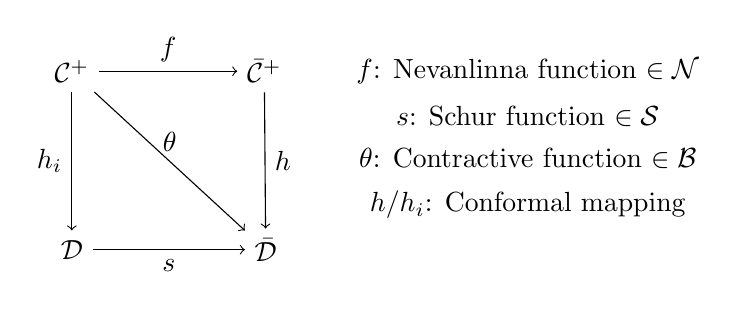
\begin{tikzpicture}[node distance=50pt]
			\node[draw=none,fill=none]  (C)  {$\C^+$};
			\node[draw=none,fill=none, right=of C]  (Cbar)  {$\Cbar^+$};                 
			\node[draw=none,fill=none, below=of C]  (D)     {$\D$};               
			\node[draw=none,fill=none,right=55pt of D]  (Dbar)  {$\Dbar$};
		
			\draw[->] (C)  -- node[above] {$f$} (Cbar) ;
			\draw[->] (C)  -- node[left] {$h_i$} (D) ;
			\draw[->] (C)  -- node[above] {$\theta$} (Dbar) ;
			\draw[->] (Cbar) -- node[right] {$h$} (Dbar) ;
			\draw[->] (D) -- node[below] {$s$} (Dbar) ;

			\node[draw=none,fill=none, right=20pt of Cbar] (f) {$f$: Nevanlinna function $\in \N$};
			\node[draw=none,fill=none, below=1pt of f]  (s)  {$s$: Schur function $\in \mathcal{S}$};                 
			\node[draw=none,fill=none, below=1pt of s]  (t)     {$\theta$: Contractive function $\in \B$};               
			\node[draw=none,fill=none,below=1pt of t]  (h)  {$h/h_i$: Conformal mapping};
		\end{tikzpicture}
	\end{minipage}
	\caption{Conformal mappings}
	\label{fig:conformal-map}
\end{figure}

Now we are ready to disscuss the Green's functions. The Lehmann 
representation of Green's function $G(z)$ is:
\begin{equation}\label{eq:Lehmann-GF-Masubara}
	G(z) = \frac{1}{Z} \sum_{nm} |A_{nm}|^2
		\frac{e^{-\beta E_n} \pm e^{-\beta E_m} }{z - E_m + E_n}
\end{equation}
where the "$+$" sign is for fermionic Green's functions and 
"$-$" sign is for bosonic Green's functions.

In fermionic case, if we take $z = x + iy$ with $y>0$, 
i.e. $z\in \C^+$, we can easily prove that $\im G(z) \leq 0$.
Therefore $-G(z) \in \N$ is an Nevanlinna function.

While the bosonic case is less trivial. 
%The real part of bosonic Green's function is:
%\begin{equation}\label{eq:real-bose-GF}
%	\re G(z) = \frac{1}{Z} \sum_{nm} 
%		\frac{|A_{nm}|^2(x - E_m + E_n)}{(x - E_m + E_n)^2 + y^2}
%		(e^{-\beta E_n} - e^{-\beta E_m}) 
%\end{equation}
The imaginary part of bosonic Green's function is:
\begin{equation}\label{eq:imag-bose-GF}
	\im G(z) = \frac{1}{Z} \sum_{nm}
		\frac{y |A_{nm}|^2 e^{-\beta E_m}}{(x - E_m + E_n)^2 + y^2}
		[(1 - e^{\beta(E_m - E_n)} ]
\end{equation}
which is negative when $E_m > E_n$ and positive when $E_m < E_n$. 
We can construct a $\tilde{G}(z)$ like:
\begin{equation}\label{eq:Lehmann-construc-GF}
	\tilde{G}(z) = \frac{1}{Z} \sum_{nm}
		\frac{|A_{nm}|^2}{z - E_m + E_n}
		\frac{e^{-\beta E_n} - e^{-\beta E_m} }{E_m - E_n}
\end{equation}
and $-\tilde{G}(z) \in \N$ is a Nevanlinna function.


%=====================================================================
\section{Hardy basis optimization}
\label{sec:hardy-basis-optimization}



\appendix
%=====================================================================
%=====================================================================
\section{Conformal transforms}
\label{app:conformal-transforms}

\subsection{The linear fractional transform}
\label{appsub:linear-fractional-transform}
The linear fractional transform is:
\begin{equation}\label{eq:linear-fractional-transform}
	\xi(z, \Y) = \frac{z - \Y}{1 - z\Y^*}
\end{equation}

It is a one to one mapping of the open unit disk $\D$ onto 
itself and a one to one mapping of the unit circle $\mathcal{T}$.
It maps point $\Y$ to the center of $\D$.


\subsection{The Mobius transform}
\label{appsub:mobius-transform}
The mapping from $\C^+/\bar{\C^+}$ to 
$\D^+/\bar{\D^+}$ is called Mobius transform.
It has the form:
\begin{equation}\label{eq:def-mobius-transform}
	h(z, \Y)  = \frac{z - \Y}{z - \Y^*}
\end{equation}
where $\Y \in \Cbar^+$ and $\Y \neq 0$. We can easily prove that 
$|h(z, \Y)| \leq 1$ for $z \in \Cbar^+$ and
$|h(z, \Y)| = 1$ if $z$ is real. $h(z, \Y)$ maps $\Y \in \Cbar^+$
to the center of the unit disk $\D$ and the real axis as the 
edge of $\Dbar$, the rest part of upper half complex plane is 
wrapped inside the unit disk. If $ \tilde{z} \in \D$, the inverse 
transform is:
\begin{equation}\label{eq:def-inv-mobius-transform}
	h^{-1}(\tilde{z}, \Y) = \frac{\Y - \tilde{z}\Y^*}{1 - \tilde{z}}
\end{equation}
Angin one can prove 
$\im h^{-1}(\tilde{z}, \Y) = (\im\Y)(1 - |\tilde{z}|^2 ) > 0$.

Proof of $|h(z, \Y)| \leq 1$ for $z \in \Cbar^+$ and
$|h(z, \Y)| = 1$ if $z$ is real. 
We already know that $\im z \geq 0,  \im \Y >0$.
\begin{align}
\begin{split}
|h(z, \Y)|^2 &= \frac{z - \Y}{z - \Y^*} \frac{z^* - \Y^*}{z^* - \Y} 
	  = \frac{|z|^2 + |\Y|^2 - z\Y^* - z^*\Y}{|z|^2 + |\Y|^2 - z\Y - z^*\Y^*}\\
	& = \frac{|z|^2 + |\Y|^2 - 2(\re z \re \Y  + \im z \im \Y)}
		{|z|^2 + |\Y|^2 - 2(\re z \re \Y  - \im z \im \Y)}
\end{split}
\end{align}
If $\im z = 0$, $|h(z, \Y)|^2 = 1$. If $\im z > 0$, $|h(z, \Y)|^2 < 1$.
And we notice that if $\im \Y = 0$, we map all points in $\Cbar$ to 
point $1$ except for point $\Y$ itself.

\bibliographystyle{unsrt} %引用顺序
\bibliography{nevanlinna.bib}
\end{document}